%\documentstyle[twocolumn,epsfig]{IEEEtran}
\documentclass[mathserif]{beamer}
% \input{amssym.def}
% \input{amssym.tex}
% \newcommand{\domain}[1]{\Bbb{#1}}
\usepackage{algorithm,algorithmic}
\usepackage{times}
\usepackage{cite}
\usepackage{graphicx}
\usepackage{amssymb,amsmath,amsthm}
\usepackage{wasysym}
\usepackage{url}
\usepackage{subfigure}
% \setcounter{page}{100}
%\usepackage{eulervm}
\usepackage{pgf}

\newcommand{\domain}[1]{\mathbb{#1}}
\renewcommand{\algorithmiccomment}[1]{ /* #1 */}

\DeclareGraphicsRule{.gif}{eps}{.gif.bb}{`gif2eps #1}

\title{Convex Fitting Using B-Spline}
\subtitle{(Project Proposal)}

\author{Wai-Shing Luk%
  \thanks{{\tiny Microelectronics Department,
      Fudan University.
      Email: luk@fudan.edu.cn}},
}

\begin{document}
\frame{\titlepage }

\frame{\frametitle{Agenda}
  \tableofcontents
}

\section{Introduction}
\frame{\frametitle{Introduction}
  \begin{itemize}
    \item
      Problem: find a posynomial/convex function that fits a set of data.
    \item
      Requirements:
      \begin{itemize}
        \item
          Smoothness, easy to evaluate.
      \end{itemize}
    \item
      Motivation:
      \begin{itemize}
        \item
          Geometric Programming (GP): Analog
          Circuit Sizing
      \end{itemize}
  \end{itemize}
}

\section{Previous Works}
\frame{\frametitle{Previous Works}
  \begin{itemize}
    \item
      Posynomial fitting
    \item
      Sum-of-squares polynomial fitting (Magnani, Lall and Boyd, CDC-ECC'05)
    \item
      Convex piecewise linear fitting (Magnani and Boyd, Technical Report, 2006)
    \item
      ConvexFit (Roy and Chen, ICCAD'05)
    \item
      ConvexSmooth (Roy and Chen, ISQED'06)
  \end{itemize}
}

\frame{\frametitle{Posynomial Fitting}
  \begin{itemize}
    \item
      Useful when need to further build more complicated posynomial functions.
    \item
      This problem is hard - in the sense that
      \begin{itemize}
        \item
          no convex programming formulation is known for this problem.
        \item
          No known orthogonal set of posynomials.
        \item
          Will not include in this proposal.
      \end{itemize}
    \item
      Prefer direct fitting to a convex function.
  \end{itemize}
}

\frame{\frametitle{SOS Fitting (CDC-ECC'05)}
  \begin{itemize}
    \item
      Let $S$ be a set of all polynomials with sum-of-squares (SOS) form.
    \item
      Fitting data restricted to this form can be formulated as a semi-definite programming (SDP),
      and hence can be solved efficiently.
    \item
      Difficulties:
      \begin{itemize}
        \item
          Not optimize among \emph{all} convex functions.
        \item
          Lack of local support (change 1 pt affect all)
        \item
          How to determine the number of terms?
        \item
          How to select the basis polynomials?
        \item
          How to evaluate the function efficiently?
      \end{itemize}
  \end{itemize}
}

\frame{\frametitle{Convex PWL Fitting}
  \begin{itemize}
    \item
      Idea: fit the data by max-affine functions $f(x) = \max\{a_i^{T} x +
      b_i\}$
    \item
      Least square fitting restricted to this form is not a convex programming; may stuck to local minimum.
    \item
      Not smooth.
  \end{itemize}
}

\frame{\frametitle{ConvexFit (ICCAD'05)}
  \begin{itemize}
    \item
      Idea: minimal adjustment of the data set such
      that its approximated Hessian matrix is
      convex (???). This problem can be formulated
      as an SDP.
    \item
      Then quadratic interpolation is used for
      smoothing the adjusted data. Disadvantages:
      \begin{itemize}
        \item
          Not guarantee that the interpolated points preserves convexity.
        \item
          Not guarantee to be smooth.
      \end{itemize}
  \end{itemize}
}

\frame{\frametitle{ConvexSmooth (ISQED'06)}
  \begin{itemize}
    \item
      Idea: retain the smoothness and
      convexity by adding extra interpolated
      points to the ConvexFit minimization process.
    \item
      Disadvantage:
      \begin{itemize}
        \item
          Very slow. Could be 100x slower than ConvexFit.
      \end{itemize}
  \end{itemize}
}


\section{Poor Man's Convex Fitting}
\frame{\frametitle{Poor Man's Convex Fitting}
  \begin{columns}
    \begin{column}{0.4\textwidth}
      \begin{itemize}
      \item
        For 1D case, use convex hull.\\
        \begin{itemize}
          \item
            Non-smooth\\
          \item
            Not fit very well, only lower bound.\\
          \item
            But at least it is convex.\\
          \item
            Hard to extent to higher dimensions.\\
        \end{itemize}
      \end{itemize}
    \end{column}

    \begin{column}{0.6\textwidth}
      \pgfputat{\pgfxy(0,-3.0)}{\pgfbox[left,base]{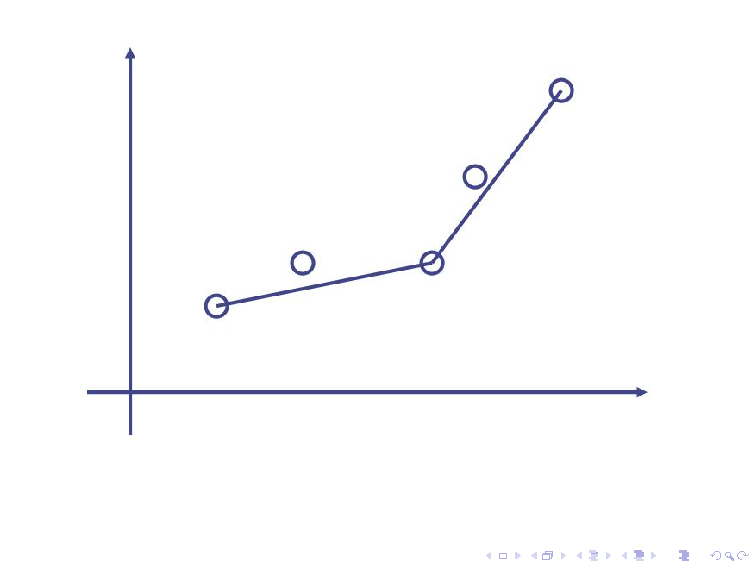
\includegraphics[width=\textwidth]{jpg2pdf1}}}
    \end{column}
  \end{columns}
}

\frame{\frametitle{Refine by B-spline}
  \begin{columns}
    \begin{column}{0.4\textwidth}
    \begin{itemize}
      \item
        Use the points lying on the convex hull as the control points.
      \item
        May further optimized by adjusting the positions of the knots (non-convex problem)
    \end{itemize}
    \end{column}

    \begin{column}{0.6\textwidth}
    \pgfputat{\pgfxy(0,-3.0)}{\pgfbox[left,base]{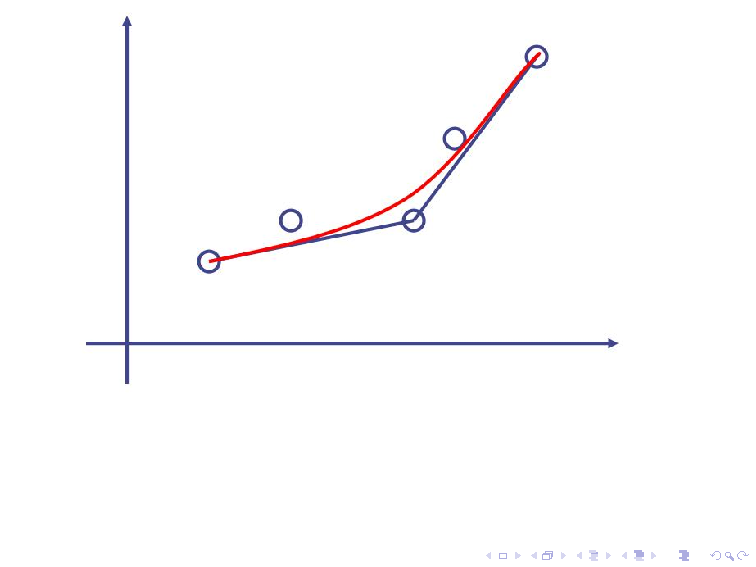
\includegraphics[width=\textwidth]{jpg2pdf2}}}
    \end{column}
  \end{columns}
}

\section{Properties of B-spline}
\frame{\frametitle{Nice Properties of B-spline }
  \begin{itemize}
    \item
      Variation Diminishing Property. Consequence of this property is that
      \alert{if all control points are in a convex hull, the
      curve is guarantee to also be convex.} 
    \item
      Function evaluation is easily obtained by a known recurrence formula.
    \item
      Derivatives (gradients) are easily obtained.
    \item
      Local support (only affect the neighbors)
    \item
      Smooth.
    \item
      Affine invariant.
  \end{itemize}
}


\section{Fitting with B-spline curve}
\frame{\frametitle{Least Squares Fit by B-spline}
\begin{columns}
  \begin{column}{0.5\textwidth}
  \begin{itemize}
    \item
      Consider convexity is not required and given
      that the positions of the knots are fixed.
    \item
      To find the optimal control points is a linear
      least squares fitting (LSF) problem and can easily
      be solved by QR method. (see MATLAB Spline Toolbox)
  \end{itemize}
  \end{column}

  \begin{column}{0.5\textwidth}
  \pgfputat{\pgfxy(0,-3.0)}{\pgfbox[left,base]{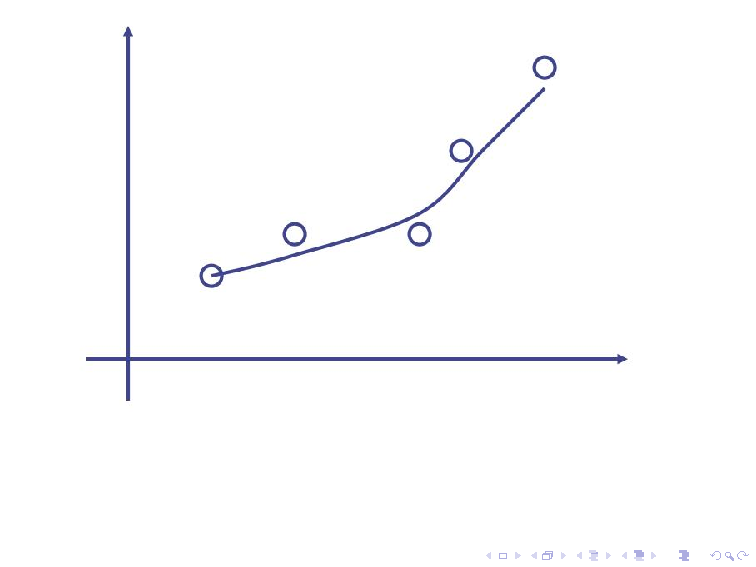
\includegraphics[width=1.2\textwidth]{jpg2pdf3}}}
  \end{column}
\end{columns}
}

\frame{\frametitle{Cvx LSF by PWL function}
\begin{columns}
  \begin{column}{0.5\textwidth}
  \begin{itemize}
    \item
      Minimize sum-of-squares error subject to all
      second divided differences $\geqslant 0$.
    \item
      Recall that
      \begin{align}
      &f[x_0,x_1,x_2] \geq 0 \nonumber\\
      &\Leftrightarrow f[x_0,x_1] \leq f[x_1,x_2] \nonumber\\
      &\Leftrightarrow \frac{f(x_1)-f(x_0)}{x_1-x_0} \leq
      \frac{f(x_2)-f(x_1)}{x_2-x_1}\nonumber
      \end{align}
    \item
      It is a convex quadratic programming (QP) with linear inequality constraints, 
      which can easily be solved.
  \end{itemize}
  \end{column}

  \begin{column}{0.5\textwidth}
  \pgfputat{\pgfxy(0,-3.0)}{\pgfbox[left,base]{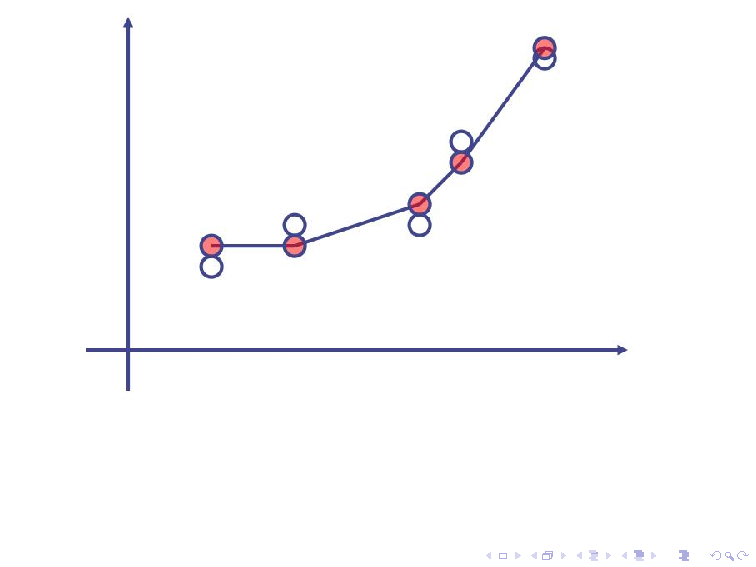
\includegraphics[width=1.2\textwidth]{jpg2pdf4}}}
  \end{column}
\end{columns}
}

\frame{\frametitle{LSF by B-spline}
\begin{columns}
  \begin{column}{0.5\textwidth}
  \begin{itemize}
    \item
      Recall that B-spline is a piecewise polynomial.
    \item
      Minimize sum-of-squares error subject to all second
      divided differences of control points $\geq 0$.
    \item
      It is still a convex quadratic programming with linear inequality constraints,
      which can easily be solved.
  \end{itemize}
  \end{column}

  \begin{column}{0.5\textwidth}
  \pgfputat{\pgfxy(0,-3.0)}{\pgfbox[left,base]{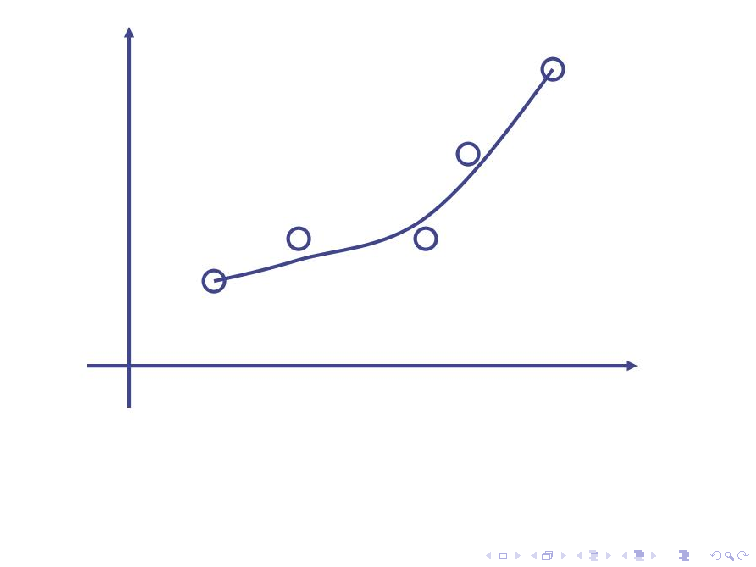
\includegraphics[width=1.2\textwidth]{jpg2pdf5}}}
  \end{column}
\end{columns}
}

\section{1-D Example}
\frame{\frametitle{B-Spline 1-D Example}
  \begin{figure}[tb]
    \centering
    \scalebox{0.5}{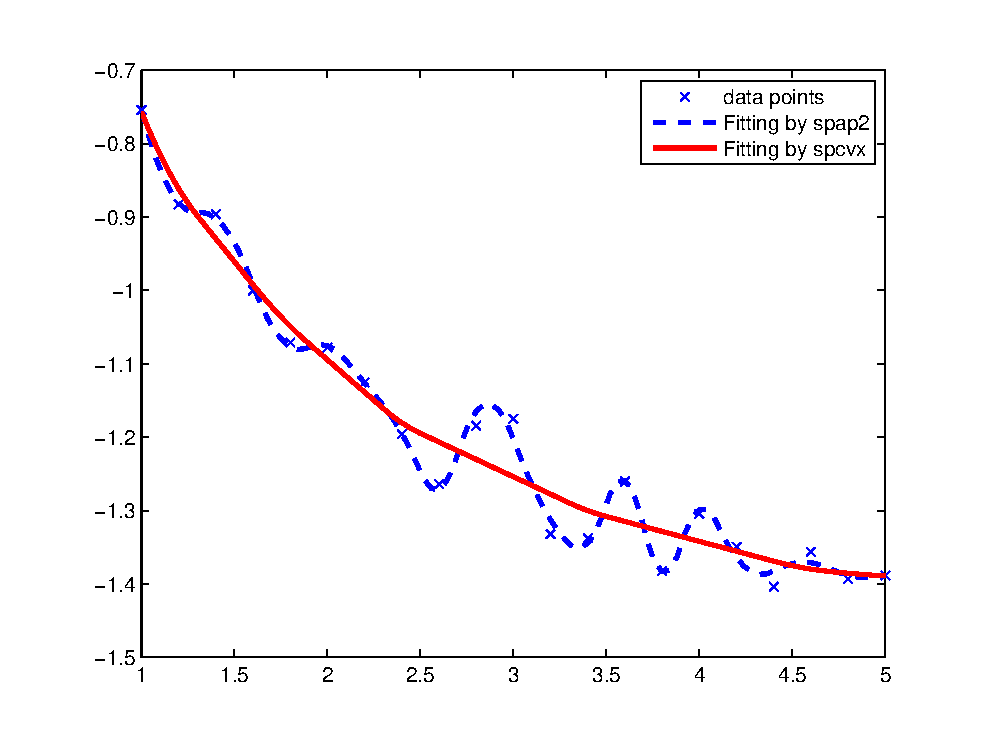
\includegraphics{cvxfit1d}}\\
    \caption{1-D Example.}\label{fig:cvxfit1d}
  \end{figure}
}

\section{2-D Example}
\frame{\frametitle{2-D Example}
  \begin{figure}[tb]
    \centering
    \scalebox{0.5}{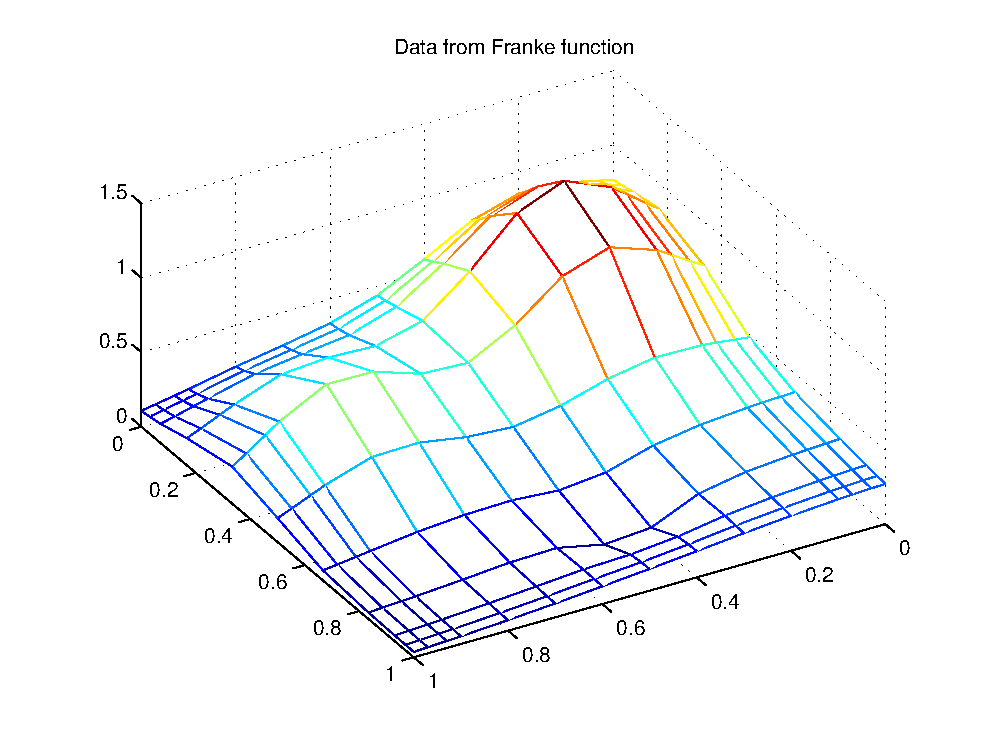
\includegraphics{franke}}\\
    \caption{Original Franke function}\label{fig:franke}
  \end{figure}
}

\frame{\frametitle{2-D Example (Cont'd}
  \begin{figure}[tb]
    \centering
    \scalebox{0.5}{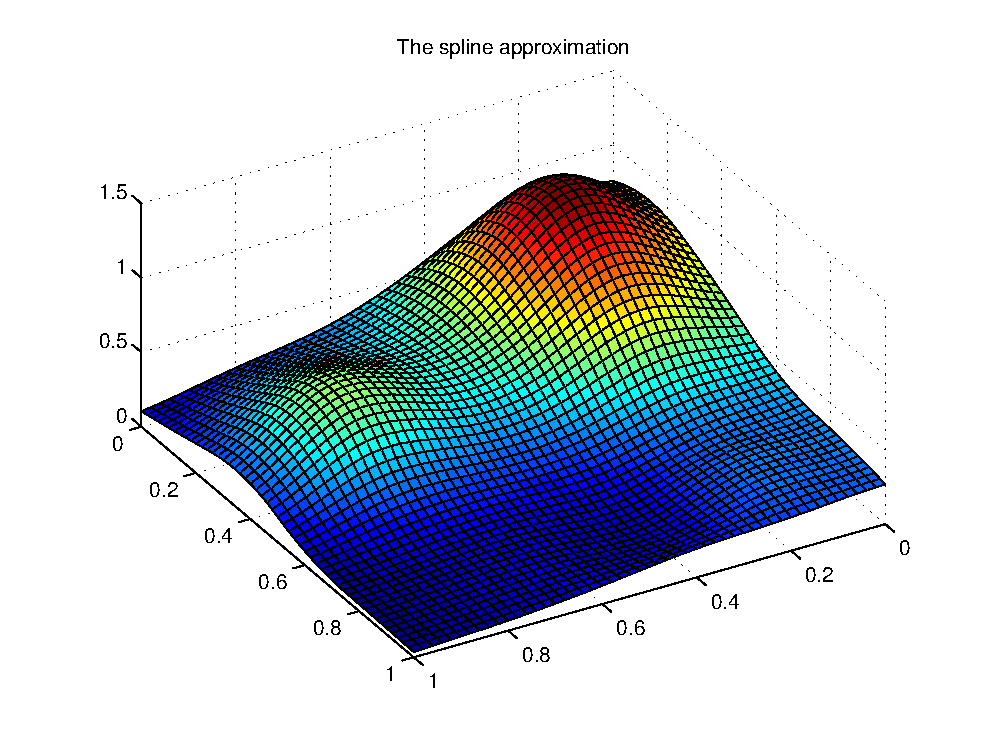
\includegraphics{spline2d}}\\
    \caption{Least squares approximation by Matlab}\label{fig:spline2d}
  \end{figure}
}

\frame{\frametitle{2-D Example (Cont'd}
  \begin{figure}[tb]
    \centering
    \scalebox{0.5}{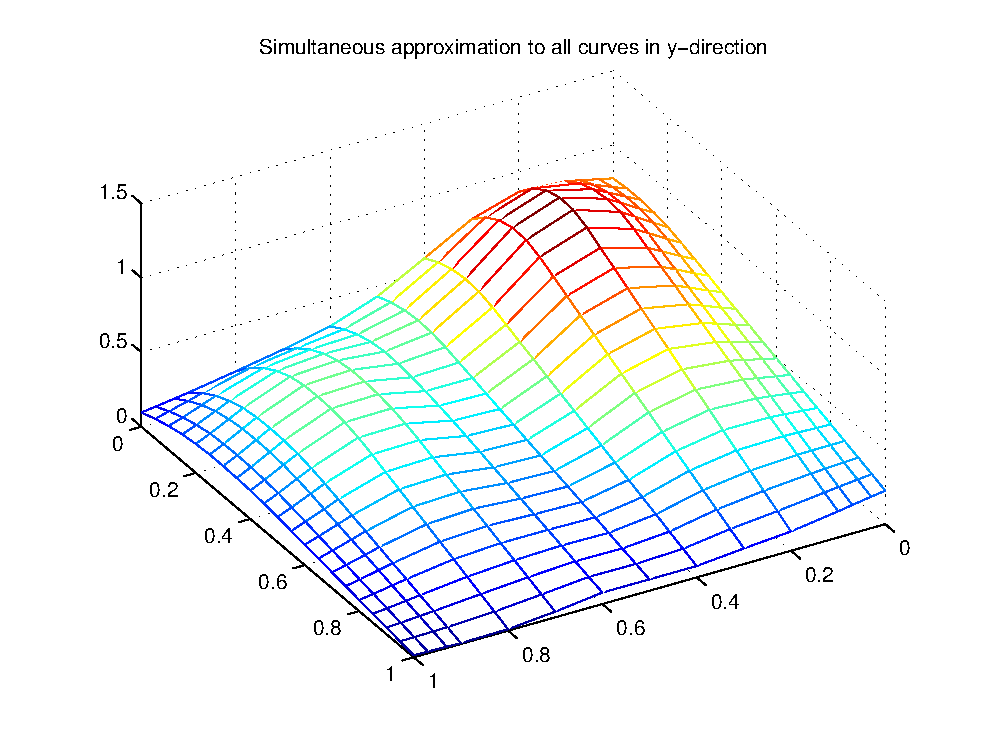
\includegraphics{spcvx_y}}\\
    \caption{Convex fitting in all y-directions 
      (precisely concave fitting here)}\label{fig:spcvx_y}
  \end{figure}
}

\frame{\frametitle{2-D Example (Cont'd}
  \begin{figure}[tb]
    \centering
    \scalebox{0.5}{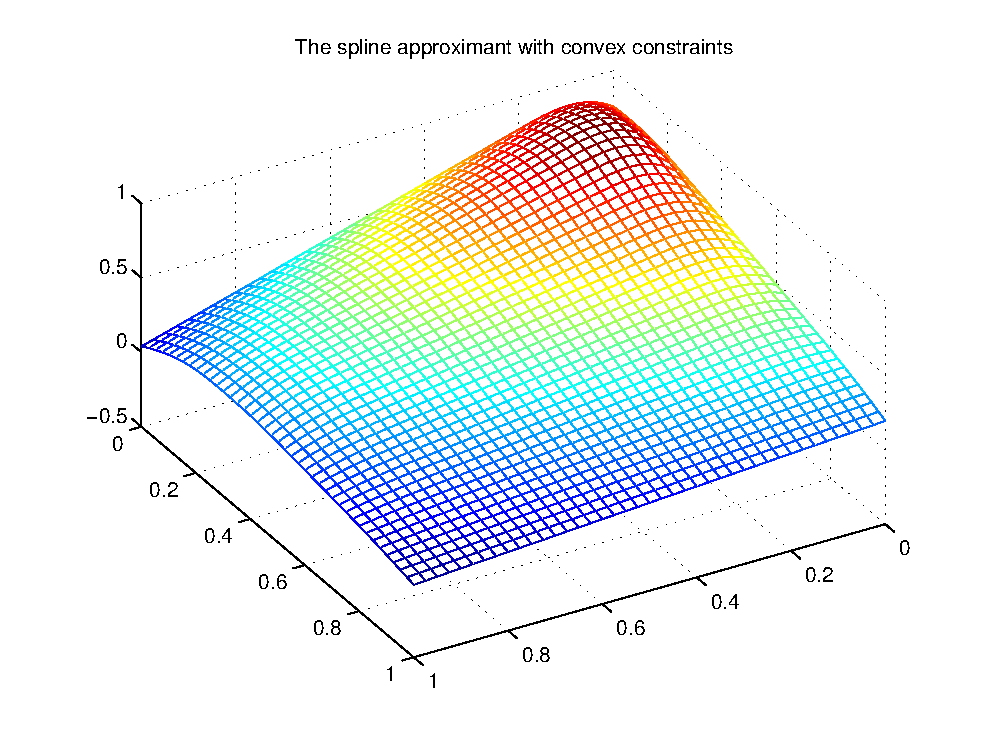
\includegraphics{spcvx_xy}}\\
    \caption{Post-Convex fitting in all x-directions}\label{fig:spcvx_xy}
  \end{figure}
  \alert{Note: does not guarantee to be concave!}
}


\frame{\frametitle{Fitting Multivariate Data with B-spline}
  \begin{itemize}
  \item
    Data in a rectangular grid: Tensor product B-spline.
  \item
    Convexity enforced in all individual dimensions (linear
    inequalities) does not guarantee to be overall convex.  
  \item
    Correct solution: Linear inequality constraint should extend to Linear
    Matrix Inequality (LMI) constraint (non-linear but still convex).
  \item
    The problem is so called semidefinite programming, that can be
    solved efficiently in principle.
  \end{itemize}
}

\frame{\frametitle{B-Spline Least Squares Fitting}
  \begin{itemize}
    \item
      Without convex restriction, least squares fitting
      by B-spline already exists in MATLAB's Spline toolbox.
    \item
      Questions:
      \begin{itemize}
        \item
          How to formulate the problem in semidefinite programming?
        \item
          How to handle process variations? (AA?)
        \item
          How to integrate to the existing GP?
      \end{itemize}
  \end{itemize}
}

\frame{\frametitle{Summary}
  \begin{center}
    \begin{tabular}{c|l|l|l|l|l}
      \hline
      & \small{CvxPWL} & \small{CvxFit} & \small{CvxSmth} & \small{SOS} & \small{B-spline} \\
      \hline
      \small{Convex formulation} & *      & ****   & ****    & ***** & *****    \\
      \hline
      \small{Smoothness}     & *  & ** & **** & ***** & ***** \\
      \hline
      \small{Convex preserve} & ***** & ** & **** & ***** & ***** \\
      \hline
      \small{Ease of fitting} & * & ***** & * & *** & ***** \\
      \hline
      \small{Ease of evaluation} & ***** & *** & *** & * & ***** \\
      \hline
      \small{Local support} & ***** & ***** & ***** & * & ***** \\
      \hline
    \end{tabular}
  \end{center}
}

\frame{\frametitle{Proposal}
  \begin{itemize}
    \item
      Beginner: Try a simple problem, say fitting $\tan^{-1}(x)$, in MATLAB.
    \item
      Intermediate: Apply the new method to our op-amp circuit sizing example.
      \begin{itemize}
        \item
          E.g. replace one constraint, say phase margin constraint,
          by Convex fitting, and re-run the ellipsoid method.
      \end{itemize}
    \item
      Advanced: Implement the method in C++. Replace ACCO optimization
      engine (differential evolution) with the new method: ellipsoid+cvxfit+evolution
    \item
      Expert level: robust design: ellipsoid+cvxfit+AA+evolution
  \end{itemize}
}


\section{Reference}

\bibliographystyle{unsrt}

\frame{\frametitle{Reference}
  \bibliography{ref-cvxfit}
  %\cite{M_Spline}
  %\cite{GMP_03}
  %\cite{IntroSpline}
}
\end{document}
